\documentclass[11pt, a4paper, twoside, italian]{article}

\usepackage{blindtext}
\usepackage{geometry}
\usepackage{setspace}
\usepackage{titlesec}
\usepackage{indentfirst}
\usepackage{graphicx}
\usepackage{babel}
\usepackage{multicol}
\usepackage{amsmath}
\usepackage{subcaption}
\usepackage[hang, flushmargin, multiple, bottom]{footmisc}
\usepackage{float}
\usepackage{array}
\usepackage{booktabs}
\usepackage{url}
\usepackage{csvsimple}
\usepackage{colortbl}
\usepackage{multicol}
\usepackage{enumerate}
\usepackage{multirow}
\usepackage{booktabs}
\usepackage{siunitx}
\usepackage{subcaption}
\usepackage[margin=0.2cm]{caption}
\usepackage{longtable}
\usepackage{physics}
\usepackage{comment}
\usepackage{listings}
\usepackage{xcolor}
\usepackage{enumitem}
\usepackage{wrapfig}
\usepackage{hyperref}
\usepackage{cleveref}
\usepackage[ddmmyyyy]{datetime}
\usepackage[export]{adjustbox}
% for watermark
\usepackage{draftwatermark}
\SetWatermarkText{
\includegraphics{../../media/img/draft_watermark.png}}

\titlespacing*{\section}{0px}{3mm}{1mm}
\titlespacing*{\subsection}{0px}{3mm}{1mm}
\geometry{
  left=2cm,
  right=2cm,
  top=2cm,
  bottom=2cm
}
\setlength{\parindent}{10mm}

\author{Edoardo Frulla}
\date{Corso "Introduzione ai sistemi complessi", I semestre a.a. 2022/2023 \\ \vspace{0.3cm} \today}
\title{Sincronizzazione di due pendoli accoppiati}  


\definecolor{codegreen}{rgb}{0,0.6,0}
\definecolor{codegray}{rgb}{0.5,0.5,0.5}
\definecolor{codepurple}{rgb}{0.58,0,0.82}
\definecolor{backcolour}{rgb}{0.95,0.95,0.92}
  
\lstdefinestyle{mystyle}{
  backgroundcolor=\color{backcolour},   
  commentstyle=\color{codegreen},
  keywordstyle=\color{magenta},
  numberstyle=\tiny\color{codegray},
  stringstyle=\color{codepurple},
  basicstyle=\ttfamily\footnotesize,
  breakatwhitespace=false,         
  breaklines=true,                 
  captionpos=b,                    
  keepspaces=true,                 
  numbers=left,                    
  numbersep=5pt,                  
  showspaces=false,                
  showstringspaces=false,
  showtabs=false,               
  tabsize=2,
  inputencoding = utf8,  % Input encoding
  extendedchars = true,  % Extended ASCII
  literate      =        % Support additional characters
    {á}{{\'a}}1  {é}{{\'e}}1  {í}{{\'i}}1 {ó}{{\'o}}1  {ú}{{\'u}}1
    {Á}{{\'A}}1  {É}{{\'E}}1  {Í}{{\'I}}1 {Ó}{{\'O}}1  {Ú}{{\'U}}1
    {à}{{\`a}}1  {è}{{\`e}}1  {ì}{{\`i}}1 {ò}{{\`o}}1  {ù}{{\`u}}1
    {À}{{\`A}}1  {È}{{\`E}}1  {Ì}{{\`I}}1 {Ò}{{\`O}}1  {Ù}{{\`U}}1
    {ä}{{\"a}}1  {ë}{{\"e}}1  {ï}{{\"i}}1 {ö}{{\"o}}1  {ü}{{\"u}}1
    {Ä}{{\"A}}1  {Ë}{{\"E}}1  {Ï}{{\"I}}1 {Ö}{{\"O}}1  {Ü}{{\"U}}1
    {â}{{\^a}}1  {ê}{{\^e}}1  {î}{{\^i}}1 {ô}{{\^o}}1  {û}{{\^u}}1
    {Â}{{\^A}}1  {Ê}{{\^E}}1  {Î}{{\^I}}1 {Ô}{{\^O}}1  {Û}{{\^U}}1
    {œ}{{\oe}}1  {Œ}{{\OE}}1  {æ}{{\ae}}1 {Æ}{{\AE}}1  {ß}{{\ss}}1
    {ẞ}{{\SS}}1  {ç}{{\c{c}}}1 {Ç}{{\c{C}}}1 {ø}{{\o}}1  {Ø}{{\O}}1
    {å}{{\aa}}1  {Å}{{\AA}}1  {ã}{{\~a}}1  {õ}{{\~o}}1 {Ã}{{\~A}}1
    {Õ}{{\~O}}1  {ñ}{{\~n}}1  {Ñ}{{\~N}}1  {¿}{{?`}}1  {¡}{{!`}}1
    {°}{{\textdegree}}1 {º}{{\textordmasculine}}1 {ª}{{\textordfeminine}}1
    {£}{{\pounds}}1  {©}{{\copyright}}1  {®}{{\textregistered}}1
    {«}{{\guillemotleft}}1  {»}{{\guillemotright}}1  {Ð}{{\DH}}1  {ð}{{\dh}}1
    {Ý}{{\'Y}}1    {ý}{{\'y}}1    {Þ}{{\TH}}1    {þ}{{\th}}1    {Ă}{{\u{A}}}1
    {ă}{{\u{a}}}1  {Ą}{{\k{A}}}1  {ą}{{\k{a}}}1  {Ć}{{\'C}}1    {ć}{{\'c}}1
    {Č}{{\v{C}}}1  {č}{{\v{c}}}1  {Ď}{{\v{D}}}1  {ď}{{\v{d}}}1  {Đ}{{\DJ}}1
    {đ}{{\dj}}1    {Ė}{{\.{E}}}1  {ė}{{\.{e}}}1  {Ę}{{\k{E}}}1  {ę}{{\k{e}}}1
    {Ě}{{\v{E}}}1  {ě}{{\v{e}}}1  {Ğ}{{\u{G}}}1  {ğ}{{\u{g}}}1  {Ĩ}{{\~I}}1
    {ĩ}{{\~\i}}1   {Į}{{\k{I}}}1  {į}{{\k{i}}}1  {İ}{{\.{I}}}1  {ı}{{\i}}1
    {Ĺ}{{\'L}}1    {ĺ}{{\'l}}1    {Ľ}{{\v{L}}}1  {ľ}{{\v{l}}}1  {Ł}{{\L{}}}1
    {ł}{{\l{}}}1   {Ń}{{\'N}}1    {ń}{{\'n}}1    {Ň}{{\v{N}}}1  {ň}{{\v{n}}}1
    {Ő}{{\H{O}}}1  {ő}{{\H{o}}}1  {Ŕ}{{\'{R}}}1  {ŕ}{{\'{r}}}1  {Ř}{{\v{R}}}1
    {ř}{{\v{r}}}1  {Ś}{{\'S}}1    {ś}{{\'s}}1    {Ş}{{\c{S}}}1  {ş}{{\c{s}}}1
    {Š}{{\v{S}}}1  {š}{{\v{s}}}1  {Ť}{{\v{T}}}1  {ť}{{\v{t}}}1  {Ũ}{{\~U}}1
    {ũ}{{\~u}}1    {Ū}{{\={U}}}1  {ū}{{\={u}}}1  {Ů}{{\r{U}}}1  {ů}{{\r{u}}}1
    {Ű}{{\H{U}}}1  {ű}{{\H{u}}}1  {Ų}{{\k{U}}}1  {ų}{{\k{u}}}1  {Ź}{{\'Z}}1
    {ź}{{\'z}}1    {Ż}{{\.Z}}1    {ż}{{\.z}}1    {Ž}{{\v{Z}}}1
    % ¿ and ¡ are not correctly displayed if inconsolata font is used
    % together with the lstlisting environment. Consider typing code in
    % external files and using \lstinputlisting to display them instead.      
    % reference to this answer https://tex.stackexchange.com/questions/24528/having-problems-with-listings-and-utf-8-can-it-be-fixed
    % and https://tex.stackexchange.com/questions/105672/special-characters-in-input-file
}

\lstset{style=mystyle}

\sisetup{separate-uncertainty=true}
%per mettere il più meno

\begin{document}
\maketitle
    \begin{abstract}
        In questo documento si introduce il fenomeno emergente della sincronizzazione.
        Si sceglie poi il sistema di due pendoli accoppiati per analizzare le caratteristiche
        dinamiche che portano alla sincronizzazione stessa, confermando l'ipotesi che
        la causa del fenomeno sia la differenza tra i tassi di dissipazione dei principali
        modi normali di oscillazione.
    \end{abstract}

\section{Introduzione}
La sincronizzazione è un particolare fenomeno che si manifesta in natura in differenti modalità: ne sono esempi gli sciami di lucciole che tendono a lampeggiare all'unisono, le cellule del cuore umano che emettono impulsi elettrici in fase permettendo le contrazioni cardiache, gli applausi che si sviluppano nel pubblico durante le opere teatrali e i neuroni che emettono segnali elettrici, amplificandone gli effetti, durante gli episodi di epilessia.
In tutti questi casi sono considerate situazioni in cui i singoli elementi che causano il fenomeno, a cui è associata una grandezza caratteristica che oscilla secondo un periodo proprio generalmente arbitrario, si trovano ad interagire e influenzandosi l'un l'altro giungono in qualche modo alla sincronizzazione più o meno completa dell'insieme di cui fanno parte.
Le interazioni che abbiamo descritto fino ad ora sono però manifestazione di interazioni non fondamentali dal punto di vista fisico: si tratta di fenomeni emergenti. 
Esistono però anche delle situazioni in cui la sincronizzazione è attribuibile alle interazioni fisiche fondamentali: possiamo per esempio pensare ai sistemi meccanici composti da pendoli o metronomi accoppiati.

Un problema di questo tipo fu affrontato per la prima volta nel Febbraio 1665, dal fisico Olandese Christiaan Huygens: doveva affrontare il problema di migliorare la precisione degli orologi a pendolo, anche essi da lui inventati. Si trovava nella sua stanza a causa di una "leggera indisposizione" quando si accorse che due orologi a pendolo che aveva costruito si erano spontaneamente sincronizzati, in controfase\footnote{controllare}. Provò allora, sospettando un accoppiamento dovuto al mezzo a cui si trovavano entrambi in contatto, a svolgere alcuni esperimenti, in particolare agganciandone due a un supporto in legno sospeso tra due sedie, come si nota da \cref{pendoli_huygens}.
\begin{figure}
    \centering
    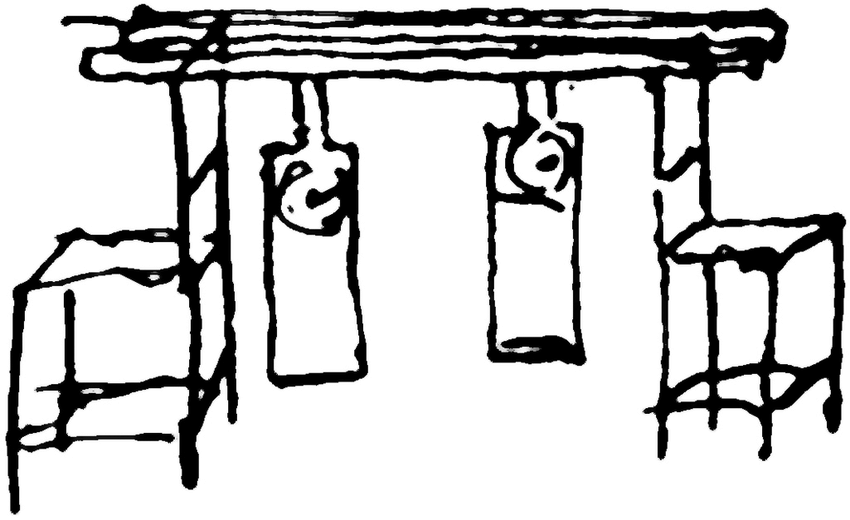
\includegraphics[width=0.4\textwidth]{../../media/img/pendolums.png}
    \caption{\textit{Schema della situazione sperimentale disegnato da Huygens. I due orologi sono sospesi a un supporto comune.}}
    \label{pendoli_huygens}
\end{figure}
Un problema più semplice da affrontare rispetto a quello dei due orologi a pendolo è quello di due pendoli posti su una base comune, libera di muoversi lungo un asse.
\section{Analisi meccanica del moto di due pendoli accoppiati}
\begin{figure}[h]
    \centering
    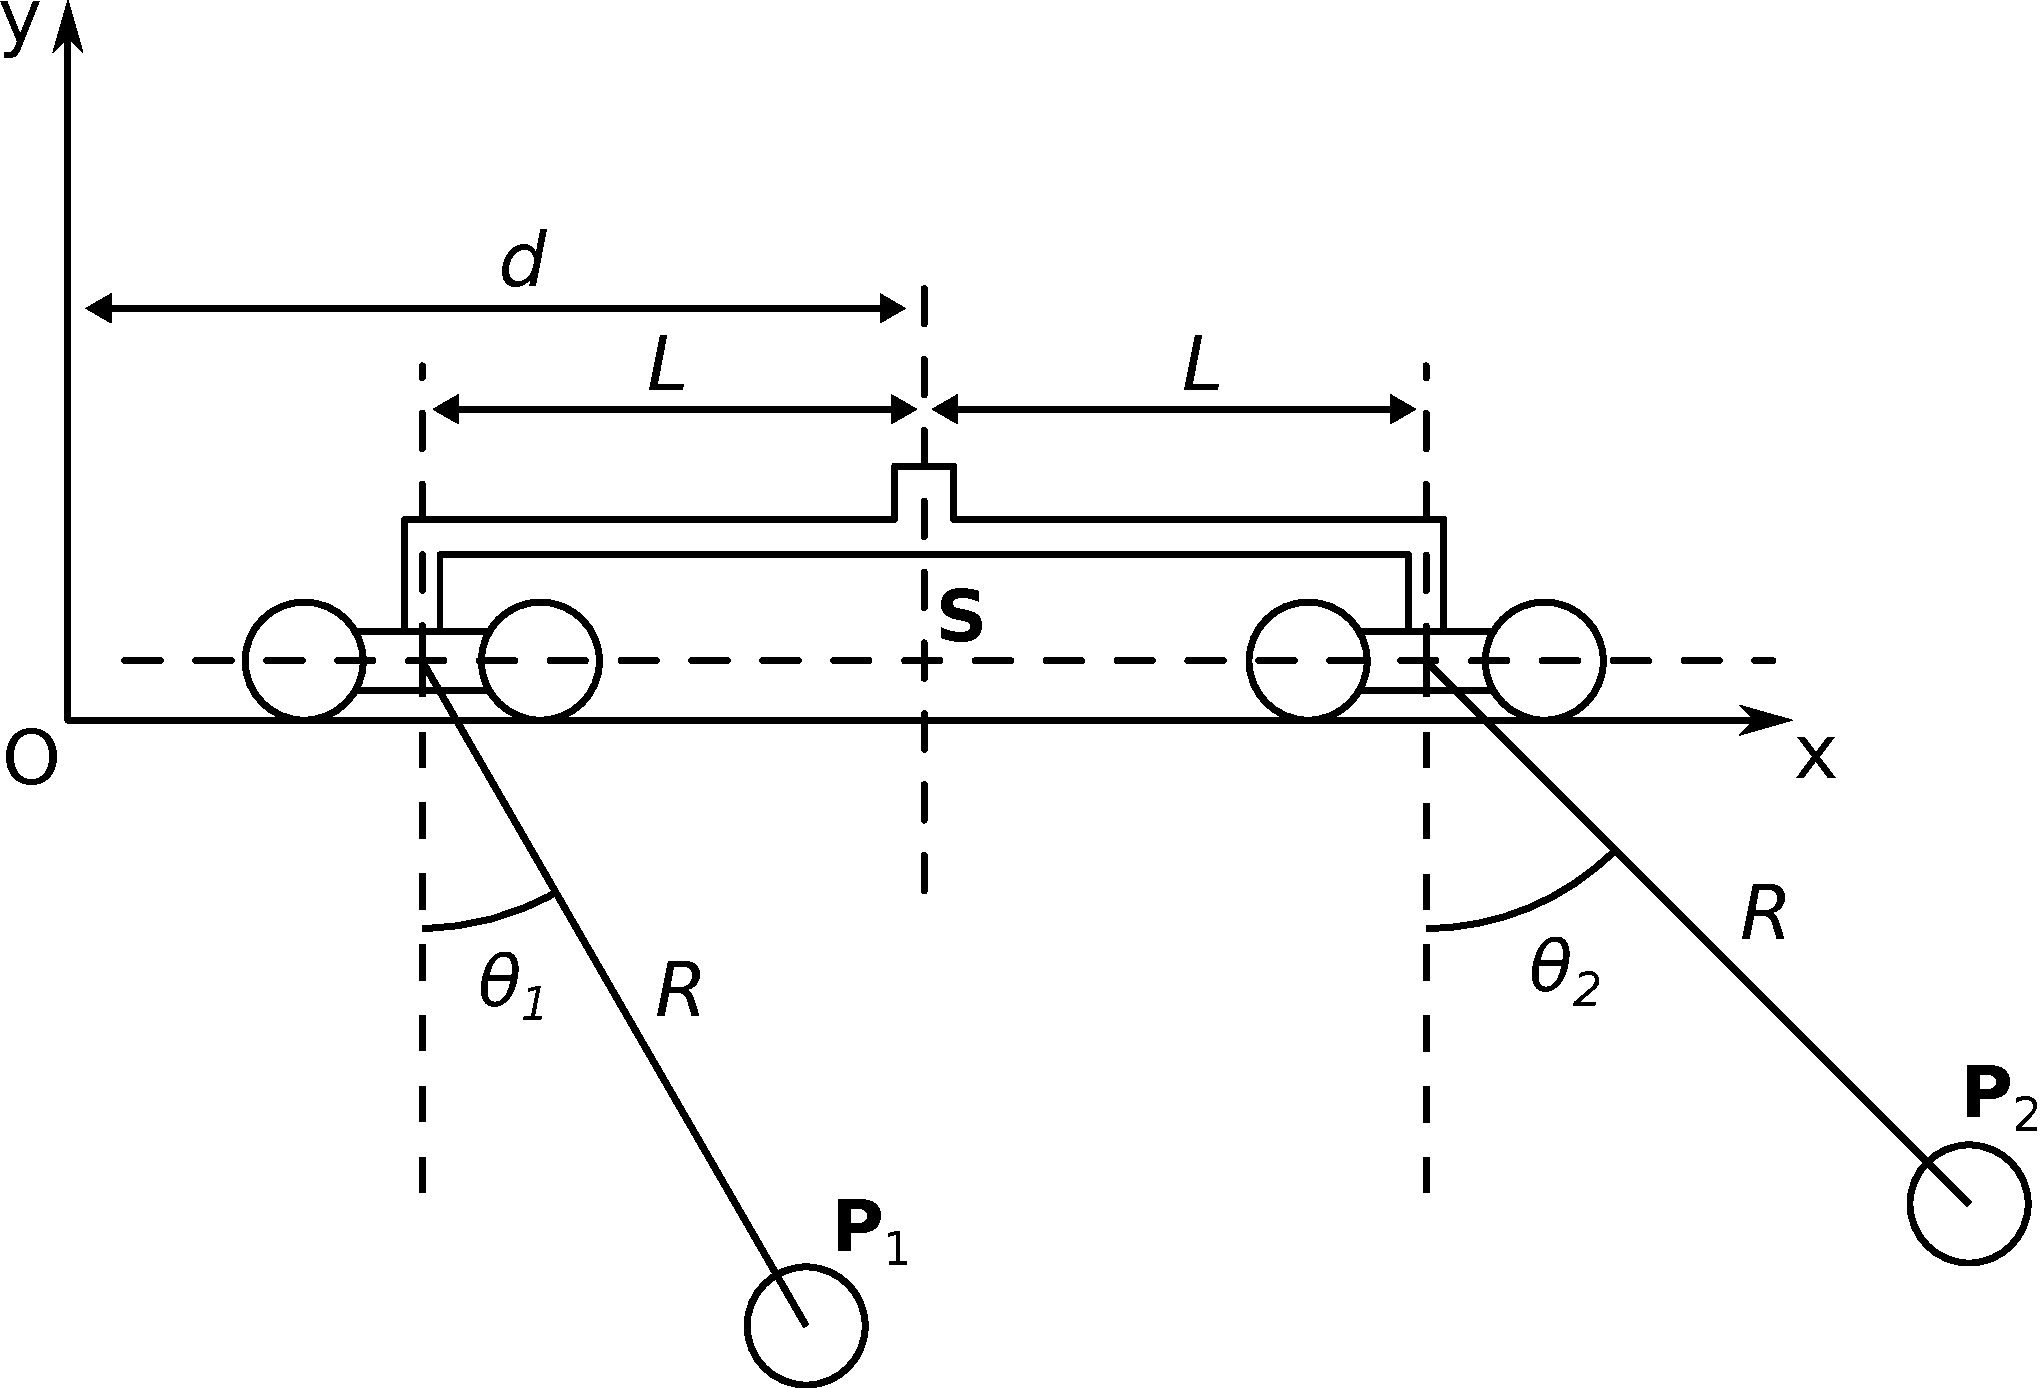
\includegraphics[width=0.5\textwidth]{../../media/cad/sketch_2.pdf}
    \caption{\textit{Modello del sistema costruito con indicate
     le grandezze rilevanti. Le lettere maiuscole in grassetto indicano dei punti, quelle in corsivo delle 
     costanti; le minuscole invece indicano le variabili.} }
    \label{pendolicorpolibero}
\end{figure}
Innanzitutto si consideri il diagramma indicato in \cref{pendolicorpolibero}.
I tre corpi coinvolti nella dinamica sono i due pendoli, il cui centro 
geometrico è indicato dai punti $\mathbf{P}_1$ e $\mathbf{P}_2$, entrambi di massa $m$,
e il supporto rigido, costituito da due carrellini identici collegati tra loro da un'asta,
indicato dal punto $\mathbf{S}$, arbitrariamente fissato lungo l'asse di simmetria del sistema 
parallelo all'asse $y$, di massa $M$. In questo caso, per comodità il punto $\mathbf{S}$ 
viene fissato lungo l'asse nel punto di intersezione con l'asse di simmetria dei carrellini
parallelo all'asse $x$.

Si assuma che il sistema sia libero di muoversi esclusivamente in un piano fissato, in questo caso
il piano $xy$, e che il moto del supporto sia ristretto alla direzione $x$ (è "appoggiato" sull'asse $x$).
Si supponga che le masse dell'asta e dei fili colleganti i carrellini tra loro
e con le masse oscillanti $\mathbf{P}$ siano trascurabili rispetto alle restanti; 
inoltre si trascurino anche le masse delle ruote dei carrellini, che, se presenti, si assume ruotino senza strisciare.
Per quanto riguarda le masse dei pendoli puntiformi, queste sono pensate fissate nel centro geometrico degli stessi.
In questo modo è possibile ottenere una notevole semplificazione della trattazione analitica,
descrivendo comunque con una buona approssimazione il moto degli elementi principali.

È possibile quindi ricavare le coordinate dei tre elementi rilevanti, ossia i due pendoli e il supporto:
\begin{gather*}
\mathbf{P}_1 = (d - L + R \sin \theta_1, S_y - R \cos \theta_1 ) \, , \\
\mathbf{P}_2 = (d + L + R \sin \theta_2, S_y - R \cos \theta_2 ) \, , \\
\mathbf{S} = (d , S_y) \, .
\end{gather*}
Calcolando quindi l'energia cinetica per ogni oggetto:
\begin{gather*}
K_{\mathbf{P}_1}=  \frac{m}{2} \lVert \dot{\mathbf{P}}_1 \rVert^2 =  \frac{m}{2}(\dot{d}^2 + R^2 \dot\theta_1^2+ 2\dot{d}R\cos\theta_1 \dot{\theta_1}) \, , \\
K_{\mathbf{P}_2} = \frac{m}{2} \lVert \dot{\mathbf{P}}_2 \rVert^2 =  \frac{m}{2}(\dot{d}^2 + R^2 \dot\theta_2^2+ 2\dot{d}R\cos\theta_2 \dot{\theta_2}) \, , \\
K_{\mathbf{S}} =  \frac{M}{2} \lVert \dot{\mathbf{S}} \rVert^2 = \frac{M}{2} \dot{d}^2 \, .
\end{gather*}
L'energia potenziale invece è:
\begin{gather*}
V_{\mathbf{P}_1}= mg P_{1y} = mg (S_y - R \cos \theta_1 ) \, , \\
V_{\mathbf{P}_2} = mg P_{2y} = mg (S_y - R \cos \theta_2 ) \, , \\
V_{\mathbf{S}} = mg S_{y} \, .
\end{gather*}
E quindi la lagrangiana del sistema si calcola, a meno di costanti, come
\begin{equation*}
\mathcal{L} = K_{TOT} - V_{TOT} = \left(m+ \frac{M}{2}\right) \dot{d}^2 + \frac{m R^2}{2}  (\dot\theta_1^2 + \dot\theta_2^2) + m \dot{d} R (\cos\theta_1 \dot\theta_1 + \cos \theta_2 \dot \theta_2) + mgR(\cos\theta_1 + \cos \theta_2) \, .
\end{equation*}
\subsection{Equazioni del moto in assenza di attrito}
Per proseguire è necessario approssimare
la lagrangiana nel regime di piccole oscillazioni:
\begin{equation}
\mathcal{L}_{PO} =  \left(m+ \frac{M}{2}\right) \dot{d}^2 + \frac{m R^2}{2}  (\dot\theta_1^2 + \dot\theta_2^2) + m \dot{d} R (\dot \theta_1 + \dot \theta_2) - \frac{m gR}{2} (\theta_1^2 + \theta_2^2) \, .
\label{lagrangianapo}
\end{equation}
Si nota immediatamente che nella lagrangiana è presente una coordinata ciclica, $d$; c'è
 quindi un integrale primo del moto, cioè una quantità che resta costante durante 
l'evoluzione temporale del sistema:
\begin{equation}
p_d = \frac{\partial \mathcal{L}_{PO}}{\partial \dot{d}} =(2m+M) \dot d + m R (\dot\theta_1 + \dot \theta_2) \, .
\label{ciclica}
\end{equation}
Si può sfruttare adesso un conveniente cambio di coordinate per gli angoli:
\begin{equation}
\setlength\arraycolsep{0pt}
\renewcommand\arraystretch{1.25}
\left\{
\begin{array}{c}
h = \theta_1 + \theta_2  \\
q = \theta_1 - \theta_2
\end{array}
\right.
,
\label{definizionehq}
\end{equation}
notando che
\begin{equation*}
  \theta_1^2 + \theta_2^2 = \frac{h^2 +q^2}{2} \, .
\end{equation*}
Le relazioni precedenti valgono anche tra le derivate.
Riscrivendo la lagrangiana si ottiene
\begin{equation*}
\mathcal{L}_{PO} =  \left(m+ \frac{M}{2}\right) \dot{d}^2 + \frac{mR^2}{4}  (\dot{h}^2 + \dot{q}^2) + m  R \dot{d}\dot{h} - \frac{mgR}{4}(h^2 + q^2) \, .
\end{equation*}
L'\cref{ciclica} inoltre diventa 
\begin{equation*}
  p_d = \frac{\partial \mathcal{L}_{PO}}{\partial \dot{d}} =(2m+M) \dot d + m R \dot h \, .
\end{equation*}
E' possibile utilizzare ora un'altra funzione, la funzione di Routh $\mathcal{R}_{PO}$, per poter eliminare 
un grado di libertà nelle equazioni del moto. Questa viene ricavata a partire dalla lagrangiana, introducendo solamente il
momento $p_d$:
\begin{equation*}
\mathcal{R}_{PO}(h,\dot h, q, \dot q, d, p_d )  = 
p_d \dot{d}(p_d, h,\dot h, q, \dot q)- \mathcal{L}(h,\dot h, q, \dot q, d, \dot{d}(p_d, h,\dot h, q, \dot q)) \, ,
\end{equation*}
dove sono state esplicitate le dipendenze dalle variabili. 
In particolare si nota che nella lagrangiana bisogna scrivere $\dot d$ sfruttando l'\cref{ciclica}.
Si ottiene immediatamente 
\begin{equation*}
  \mathcal{R}_{PO} = \frac{1}{2} \frac{(p_d -mR\dot h)^2}{2m + M}- \frac{mR^2}{4}  (\dot{h}^2 + \dot{q}^2) + \frac{mgR}{4}(h^2 + q^2) \, .
\end{equation*}
Da questa equazione si possono ricavare le equazioni del moto, le più importanti sono 
\begin{equation}
  \dot p_d = 0 \, ,
  \label{conservazione}
\end{equation}
che è ovviamente coerente con la conservazione di $p_d$ notata in \cref{ciclica}, e
\begin{equation}
  \begin{split}
  \ddot h = -\frac{\alpha}{R} h \, ,\\
  \ddot q = - \frac{g}{R} q \, ,
  \end{split}
  \label{equazionifinalinondissipate}
\end{equation}
utilizzando l'\cref{conservazione} e ponendo $\alpha = \frac{(2m + M) g}{M} $.
Con queste equazioni a disposizione si può completamente ricostruire il moto del sistema.
Si nota che, partendo da una situazione iniziale arbitraria,
la condizione di sincronizzazione in fase equivale alla richiesta che $q$ tenda a zero, mentre quella in controfase
equivale alla richiesta che $h$ tenda a zero. 
Occorre fare attenzione al fatto che però nella soluzione in \cref{equazionifinalinondissipate} sia $h$ che $q$ descrivono moti oscillatori con frequenza rispettiva
$\omega_h = \sqrt[]{\frac{\alpha}{R}}$ e $\omega_q = \sqrt[]{\frac{g}{R}}$.
Le uniche soluzioni per cui i pendoli oscillano sincronizzati sono quelle per cui una tra $h$ o $q$ è nulla
all'inizio del moto, restando quindi nulla per tutti gli istanti successivi.
Il moto evidentemente non converge ad una soluzione particolare, attraversa invece entrambe le configurazioni di sincronizzazione 
permanendo per il resto degli istanti in una combinazione delle due soluzioni.
\label{sezionesenzaattrito}

\subsection{Equazioni del moto in presenza di attrito}
\label{sezioneattrito}
Affinchè il moto converga ad una soluzione particolare, come accade nella realtà, 
è necessario tenere conto dei fenomeni dissipativi.
Potrebbe ad esempio essere considerato l'attrito che si sviluppa nel perno 
dei pendoli, quello generato dal movimento delle ruote dei
 carrelli, sia radente che volvente, e quello tra l'aria e le varie 
 componenti mobili.
Si supponga di voler includere nelle equazioni del moto un termine 
proporzionale alle velocità angolari $\dot \theta_1$ e $\dot \theta_2$, con costante comune di 
proporzionalità $\gamma$, avente le dimensioni di una frequenza. 
Riscrivendo le equazioni del moto 
per queste due variabili, ricavandole dalla lagrangiana in \cref{lagrangianapo} e semplificando i fattori in comune
si ottiene
\begin{equation*}
    R \ddot \theta_i + \ddot d = - g  \theta_i , \qquad i =1,2 
\end{equation*}
e si nota che è possibile aggiungere al secondo membro, in cui sono scritte le 
forze generalizzate, l'attrito citato sopra, agente ovviamente in verso 
opposto alla velocità:
\begin{equation*}
  R \ddot \theta_i + \ddot d = - g \theta_i  - \gamma   \dot \theta_i, \qquad i =1,2 \, .
\end{equation*}
Sostituendo la derivata dell'\cref{ciclica}
\begin{equation*}
  (2m + M) \ddot d = -mR (\ddot \theta_1 + \ddot \theta_2) 
\end{equation*} 
nell'equazione precedente si giunge alla coppia di equazioni:
\begin{equation*}
  R \ddot \theta_i -\frac{m}{2m + M}R (\ddot \theta_1 + \ddot \theta_2) 
  = - g \theta_i  - \gamma   \dot \theta_i \, , \qquad i =1,2 \, ,
\end{equation*}
che dopo qualche passaggio algebrico si possono riscrivere con le variabili
$h$ e $q$:
\begin{equation*}
  \begin{split}
  (R- \frac{2m}{2m + M}R) \ddot h + \gamma \dot h + g h  = 0 \, , \\
  R \ddot q +\gamma \dot q + g q = 0 \, .
  \end{split}
\end{equation*}
Manipolando algebricamente questa equazione, ridefinendo la costante
$\gamma$ e utilizzando le frequenze definite in precedenza si giunge infine a
\begin{equation*}
  \begin{split}
  \ddot h + \gamma \dot h + \omega_h^2 h  = 0 \, ,\\
  \ddot q +\gamma \dot q + \omega_q^2 q = 0 \, .
  \end{split}
\end{equation*}
La considerazione decisiva per osservare il fenomeno della sincronizzazione 
consiste nel considerare la costante $\gamma$ diversa per i due modi di oscillazione;
differenziando le nuove costanti con un pedice, si tiene conto di 
effetti dissipativi che influenzano in modo differente il modo di oscillazione
in fase rispetto a quello in controfase.
Le soluzioni generali di queste equazioni sono del tipo:
\begin{align}
    h(t) &= A_h e^{- \frac{\gamma_h}{2} t} \cos(\omega_h t + \beta_h) \label{equazionefinaleh} \, , \\
    q(t) &= A_q e^{- \frac{\gamma_q}{2} t} \cos(\omega_q t + \beta_q) \label{equazionefinaleq} \, ,
\end{align}
con $A_h$, $A_q$, $\beta_h$ e $\beta_q$ costanti reali.
È evidente quindi che se le costanti $\gamma$ sono diverse, l'ampiezza di uno di questi due modi va a zero più velocemente rispetto 
all'altro, sincronizzando il moto.

\section{Apparato sperimentale}
\subsection{Materiale utilizzato}

Durante l'esperimento sono stati coinvolti diversi elementi, tra cui:
\begin{enumerate}
      \item rotaia e carrellini\footnote{Attrezzatura gentilmente concessa dal liceo E.Medi di Senigallia}, mostrati in \cref{photo_crane}, con basso coefficiente di attrito solitamente
      utilizzati in esperimenti relativi alla conservazione della quantità
      di moto;
      \item due alte sedie in legno;
      \item filo di nylon trasparente;
      \item due strutture identiche, mostrate in \cref{photo_crane}, progettate autonomamente e stampate in 3D;
      \item scotch di carta;
      \item monete varie;
      \item spago da cucina;
      \item supporti in legno per spiedini.
\end{enumerate}
\begin{figure}[h!]
  \centering
\begin{minipage}[t]{0.45\textwidth}
  \centering
  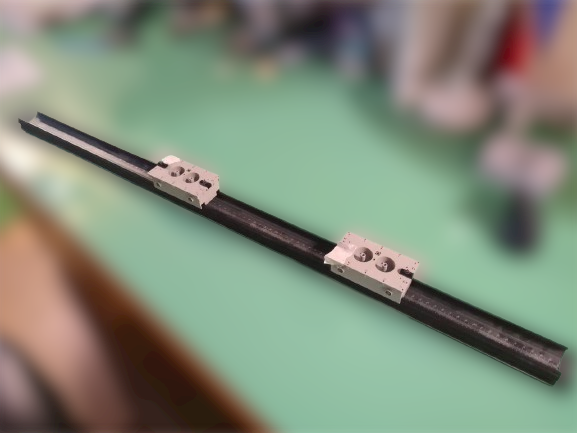
\includegraphics[valign=t, width=0.9\textwidth]{../../media/img/rail_processed.png}
  \caption{\textit{La rotaia e i carrellini presi in prestito.}}
  \label{photo_rail}
\end{minipage}
\begin{minipage}[t]{0.45\textwidth}
  \centering
  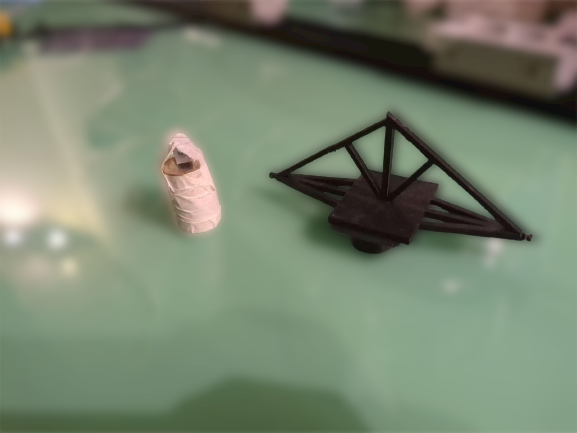
\includegraphics[valign=t, width=0.9\textwidth]{../../media/img/crane_rail-processed.png}
  \caption{\textit{Il pendolo (sinistra) e la struttura stampata in 3D dopo l'assemblaggio
  (destra).}}
  \label{photo_crane}
\end{minipage}
\end{figure}

\subsection{Strumenti di misura}

Per quanto riguarda gli strumenti di misura, sono stati invece utilizzati:
\begin{enumerate}
  \item bilancia da cucina (risoluzione \SI{1}{\g});
  \item macchina fotografica semi-professionale;
  \item treppiede per macchina fotografica;
  \item metro estendibile (risoluzione \SI{1}{\milli\m});
  \item libreria di object tracking della suite OpenCV\footnote{https://opencv.org/}.
\end{enumerate}
\subsection{Realizzazione pratica del modello}
Inizialmente la realizzazione del progetto era stata pensata tramite 
una rotaia a cuscino d'aria, per poter studiare il fenomeno, nella sua parte transiente, 
per un periodo di tempo lungo, grazie al poco attrito; questa idea però è stata abbandonata dopo alcuni tentativi per
le numerose difficoltà sperimentali. In \cref{photo_crane_air} è mostrato uno dei modelli di supporto
progettati e stampati in 3D montabili sui carrellini della rotaia.
In seguito si è provato ad usare delle costruzioni giocattolo per la creazione di una rotaia
e carrellini; purtroppo anche questo tentativo è stato accantonato a causa di 
notevoli imperfezioni e mancanza di allineamento tra i vari pezzi di rotaia. 
Un esempio di una parte della costruzione è mostrato in \cref{photo_lego}.

\begin{figure}[h!]
  \centering
\begin{minipage}{0.45\textwidth}
  \centering
  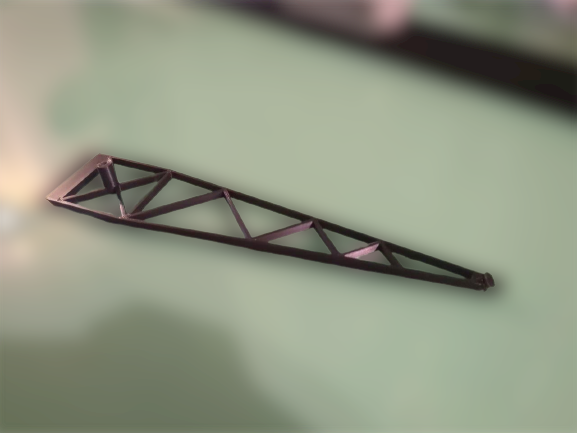
\includegraphics[width=0.9\textwidth]{../../media/img/crane_air-processed.png}
  \caption{\textit{Parte della struttura relativa alla rotaia a cuscino d'aria.}}
  \label{photo_crane_air}
\end{minipage}
\begin{minipage}{0.45\textwidth}
  \centering
  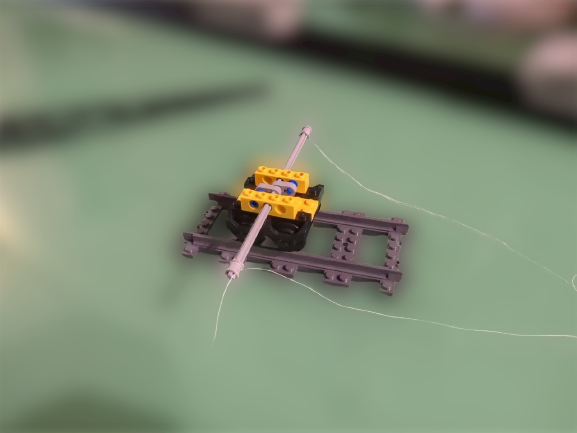
\includegraphics[width=0.9\textwidth]{../../media/img/lego_cart-processed.png}
  \caption{\textit{Il modellino realizzato a partire da costruzioni giocattolo.}}
  \label{photo_lego}
\end{minipage}
\end{figure}

In seguito si è pensato quindi di utilizzare un'altro tipo di rotaia di laboratorio, dotata
di carrellini con ruote.
La progettazione del modello si è rivolta, una volta recuperata l'apparecchiatura
di laboratorio, alla costruzione dei supporti, disegnati tramite un
software di modellizzazione tridimensionale e stampati con una stampante 3D.
Una volta stampati diversi prototipi e scelto quello migliore sono state incollate
tra loro le due parti costituenti il pezzo finale indicato in \cref{photo_crane}, i cui modelli sono mostrati
in \cref{photo_piece}, e, 
incastrato il pezzo sopra ciascun carrellino, si è costruito il supporto tramite due alte sedie
sopra le quali è stata posta la rotaia. 
\begin{figure}[h!]
  \centering
  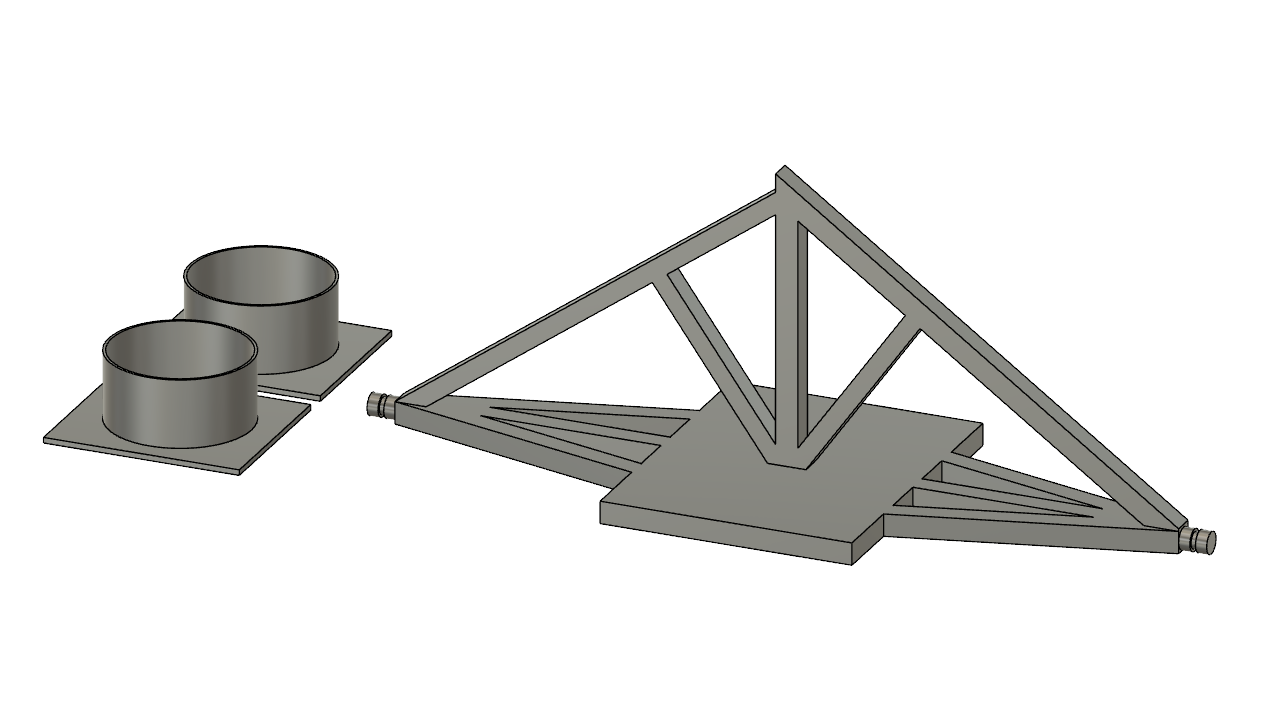
\includegraphics[width=0.9\textwidth]{../../media/img/fusion_project_cut.png}
  \caption{\textit{Le parti della struttura mostrata in \cref{photo_crane}, visualizzate nel programma
  di modellazione 3D.}}
  \label{photo_piece}
\end{figure}
È fondamentale sottolineare come si siano scelte le sedie più alte disponibili,
in quanto la lunghezza del pendolo doveva essere grande
per permettere poi l'uso dell'approssimazione di piccole oscillazioni,
non impedendo la chiara manifestazione del fenomeno della sincronizzazione.
I carrellini sono poi stati collegati tra loro tramite due bastoncini 
di legno solitamente utilizzati per la cottura degli spiedini.
La massa complessiva dei due carrellini, considerando il connettore trascurabile, è risultata essere pari a 
\SI{160 \pm 1}{\g}.
È stato controllato che lo sfondo presente dietro le
due sedie fosse inoltre fisso, ossia privo di oggetti
in movimento, per favorire il processo di tracking.
A questo punto sono stati costruiti i due pendoli identici, tramite svariate 
monete raggruppate saldamente insieme grazie all'uso dello scotch di carta, 
pesanti ciascuno \SI{139 \pm 1}{\g}.
Le monete sono state scelte per la loro elevata densità e modularità: è 
stato possibile infatti costruire diversi pendoli, di dimensioni pressochè
uguali ma di masse sensibilmente diverse gli uni dagli altri.
Sono quindi stati tagliati due pezzi approssimativamente
uguali di filo di nylon, lunghi abbastanza da sfruttare l'intera altezza 
fornita dalle due sedie, e sono poi stati agganciati ai pendoli tramite un pezzo di una nota 
marca di costruzioni giocattolo. Questi due tratti di filo sono stati poi regolati,
con l'ausilio del metro,
tramite la realizzazione di un numero adeguato di avvolgimenti nel perno di 
aggancio, fino ad ottenere una lunghezza del pendolo $R$ = \SI{85 \pm 1}{\centi\m} ciascuno (l'incertezza è 
maggiore della risoluzione del metro per tenere conto di errori nella valutazione del centro
di massa dei pendoli).
È importante notare che, per far sì che i pendoli oscillassero nello stesso piano
spaziale per tutta la durata dell'esperimento, i pendoli stessi fossero
liberi di muoversi lungo l'ansa creata dal filo di nylon appeso ai carrellini. 
A questo punto al pendolo di destra è stato collegato un breve tratto di spago 
per consentirne la manovra da una posizione che non interferisse con il tracking.
Di fronte a questa apparecchiatura, a una distanza di circa \SI{1.5}{\m}, è stato 
posizionato il treppede con sopra la macchina fotografica, per l'acquisizione
del video.
L'obiettivo della macchina fotografica è stato accuratamente posizionato, per evitare
offset prospettici in un unico verso, su un piano parallelo a quello di oscillazione dei
pendoli e la sua proiezione è stata fatta approssimativamente coincidere con il
centro della circonferenza passante per i due carrellini e i due pendoli a 
riposo.
L'apparato sperimentale completo è mostrato in \cref{setup_exp}

\begin{figure}[h!]
  \centering
  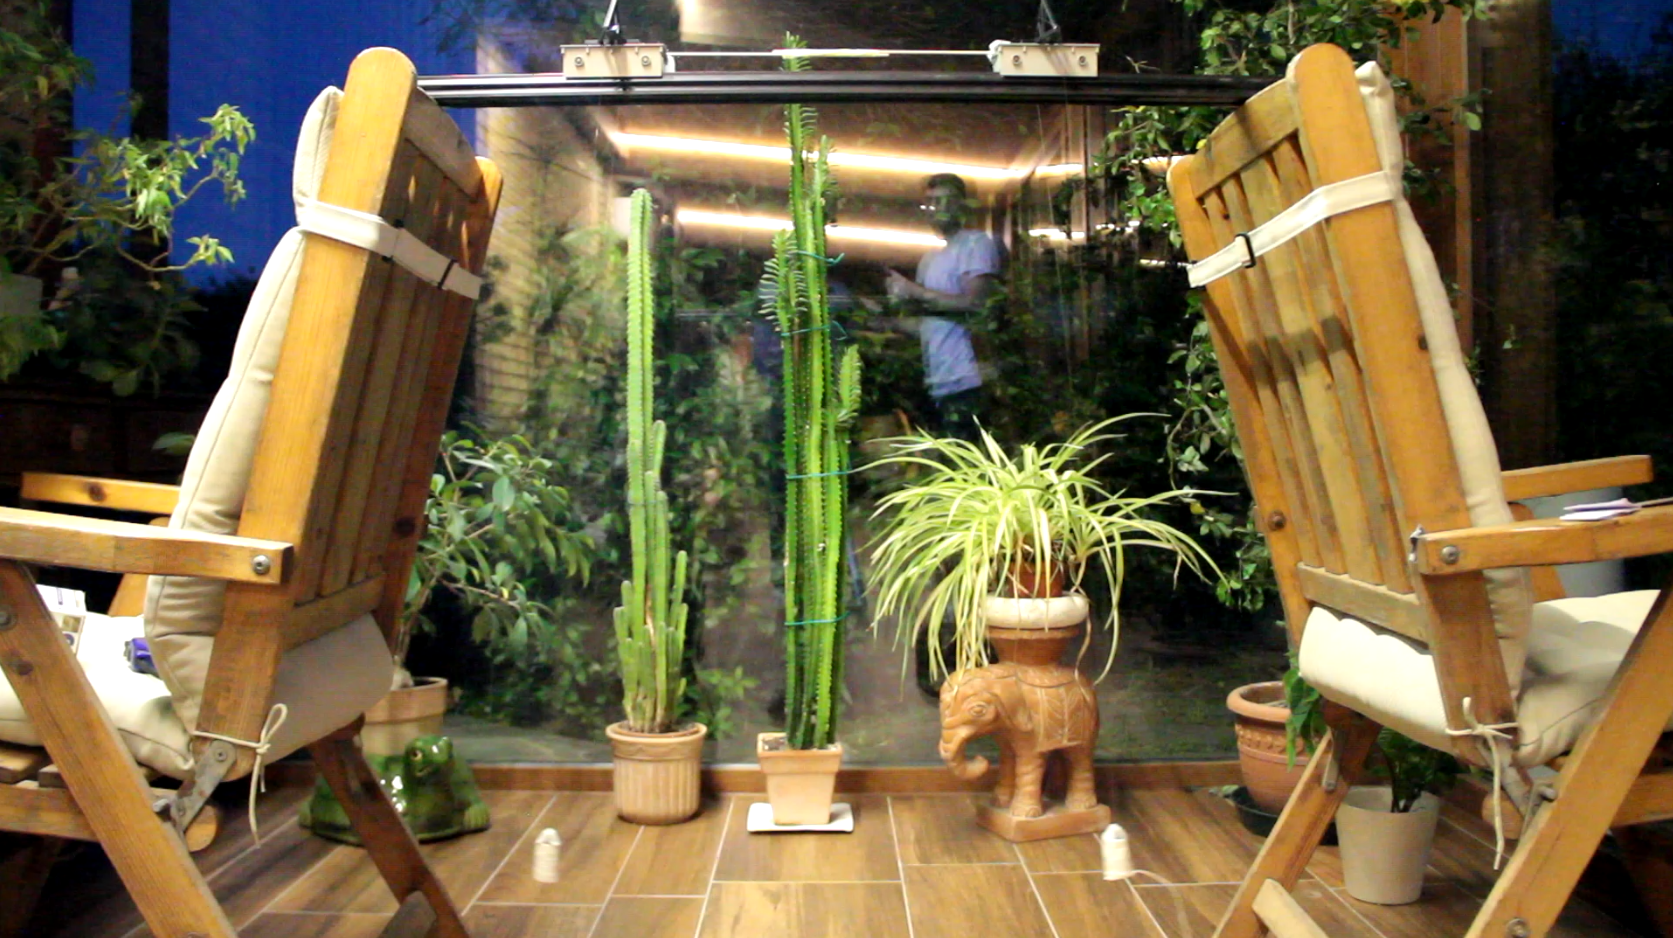
\includegraphics[width=0.6\textwidth]{../../media/img/setup_exp.png}
  \caption{\textit{Schema dell'apparato sperimentale visto dalla fotocamera.}}
  \label{setup_exp}
\end{figure}

\subsection{Esecuzione dell'esperimento}

Una volta sistemati tutti gli elementi, sono stati acquisiti differenti video del fenomeno, avendo la cura di avere una condizione
iniziale statica, con i tutti gli elementi fermi rispetto al sistema di riferimento della stanza.
Questa ipotesi è stata realizzata 
inizialmente collegando, dopo aver fermato il pendolo di sinistra, 
con un lungo spago fatto circolare attorno all'apparato, il pendolo e il carrello di destra.
In questo modo si puntava ad eliminare l'errore dato dalla non coincidenza degli istanti
di rilascio dei due elementi, che sarebbero invece stati messi in moto nello stesso momento al 
taglio dello spago.
Questo sistema, però, è risultato inadatto in quanto lo spago, una volta tagliato, continuava a 
disturbare il movimento dell'apparecchio introducendo un nuovo attrito e 
distorcendo il fenomeno.
Si è provato quindi ad agire nel modo più semplice: fermando il pendolo di sinistra, trattenendo con una mano il carrellino di destra e con l'altra lo spago 
collegato al rispettivo pendolo.
Successivamente sono stati effettuati diversi rilasci, ed è 
stato scelto per l'analisi il video in cui il pendolo e il carrellino di sinistra venivano
sganciati approssimativamente nello stesso istante.
I video sono stati registrati con la risoluzione
di 1920 x 1080 pixel, ad un framerate di 25 FPS.
\label{sezione_realizz}

\subsection{Scrittura dei programmi per l'acquisizione e l'elaborazione dati}

Per quanto riguarda la scrittura dei programmi, si è scelto di utilizzare 
la libreria OpenCV, che sta per Open Computer Vision, una libreria open source 
utilizzabile in particolare nel linguaggio di programmazione C++, 
destinata all'analisi di immagini e video. 
In questo esperimento la libreria è stata utilizzata nel per tracciare il 
movimento nel tempo dei pendoli e dei carrellini, in maniera automatizzata.
E' stato utilizzato il C++ per la nota velocità in esecuzione rispetto a 
python. Il codice è listato in \cref{listatocpp}.
Il codice inizialmente acquisisce il percorso di memorizzazione del file video, per poi 
permettere all'utente di scegliere prima l'oggetto da tracciare
 e poi 
il numero progressivo dell'acquisizione.
In seguito viene chiesto all'utente di disegnare un rettangolo attorno
all'oggetto di interesse, partendo dal suo centro.
L'algoritmo di tracking, in questo caso KCF\footnote{https://arxiv.org/abs/1404.7584}, 
inizia poi a processare i vari frame, seguendo l'oggetto e scrivendo nel file
le coordinate in pixel del centro del rettangolo (l'origine è nell'angolo in alto a sinistra e gli assi 
sono diretti verso destra e verso il basso).
Vari momenti del processo appena descritto sono mostrati in \cref{photo_tracking}.

\begin{figure}[h!]
  \centering
\begin{minipage}{0.3\textwidth}
  \centering
  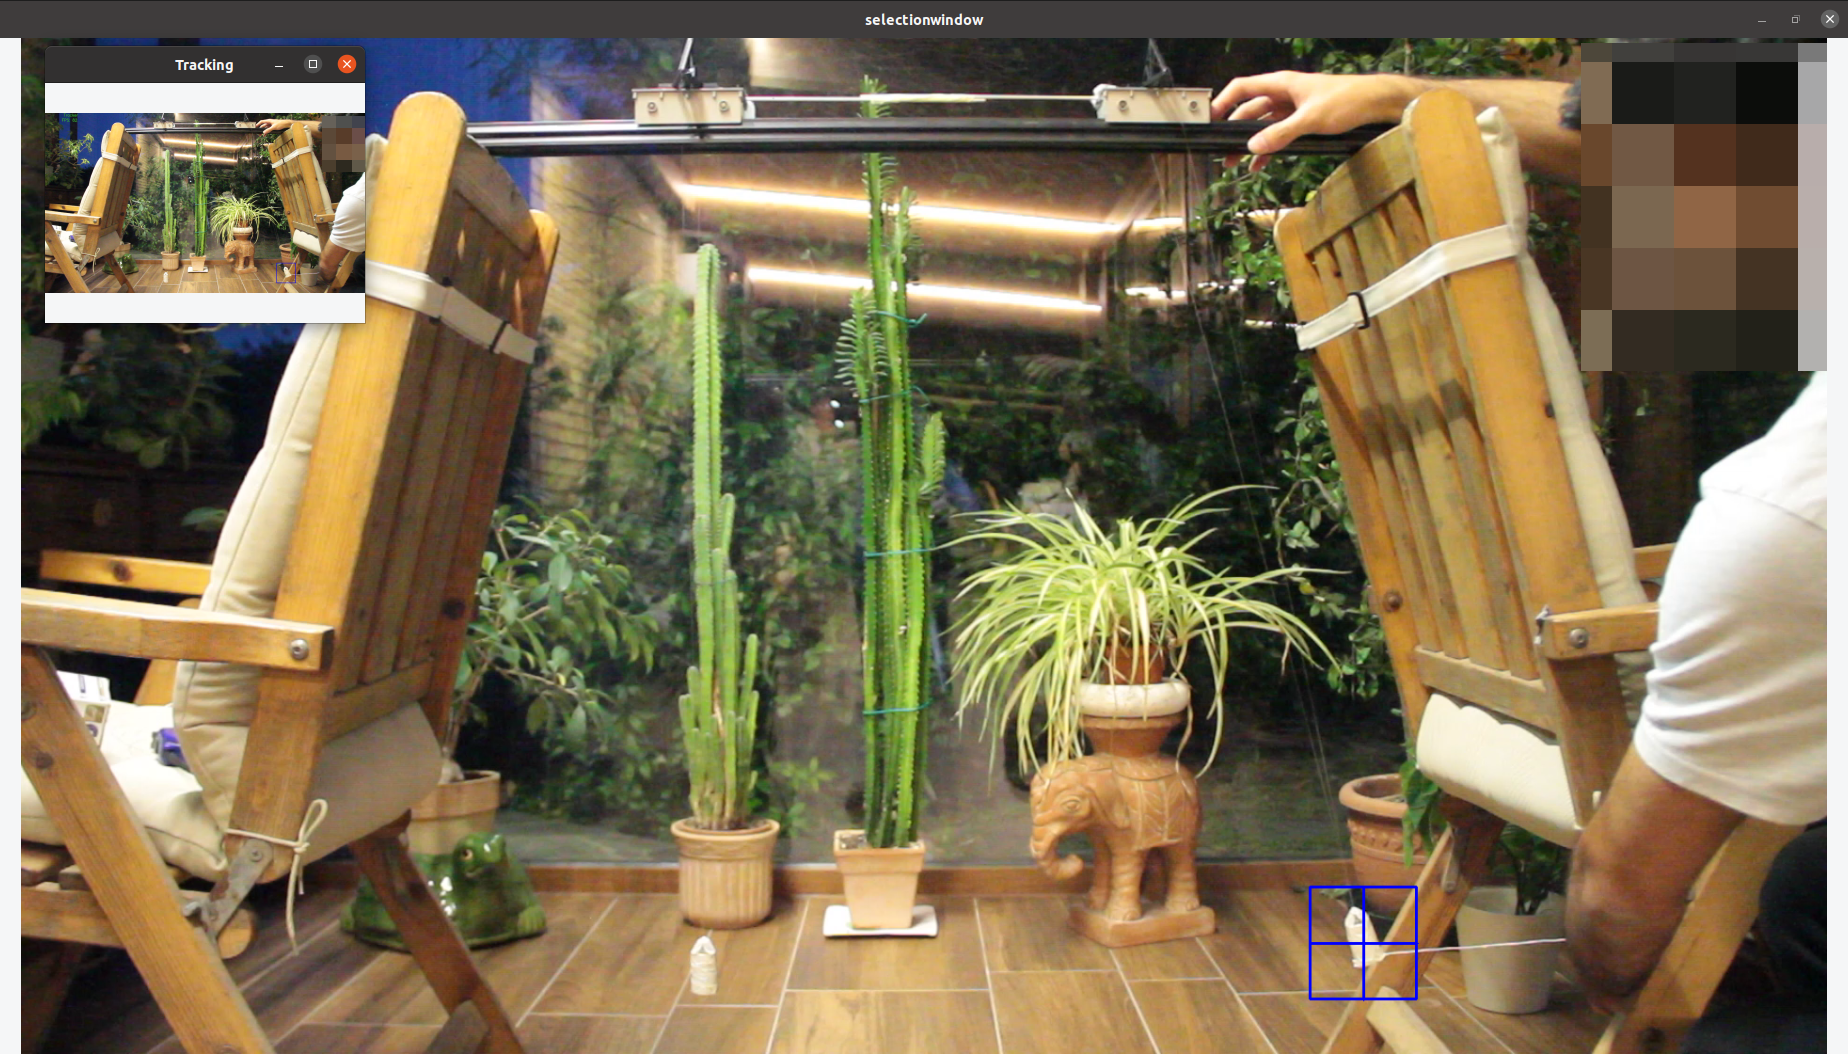
\includegraphics[width=0.9\textwidth]{../../media/img/tracking_1.png}
\end{minipage}
\begin{minipage}{0.3\textwidth}
  \centering
  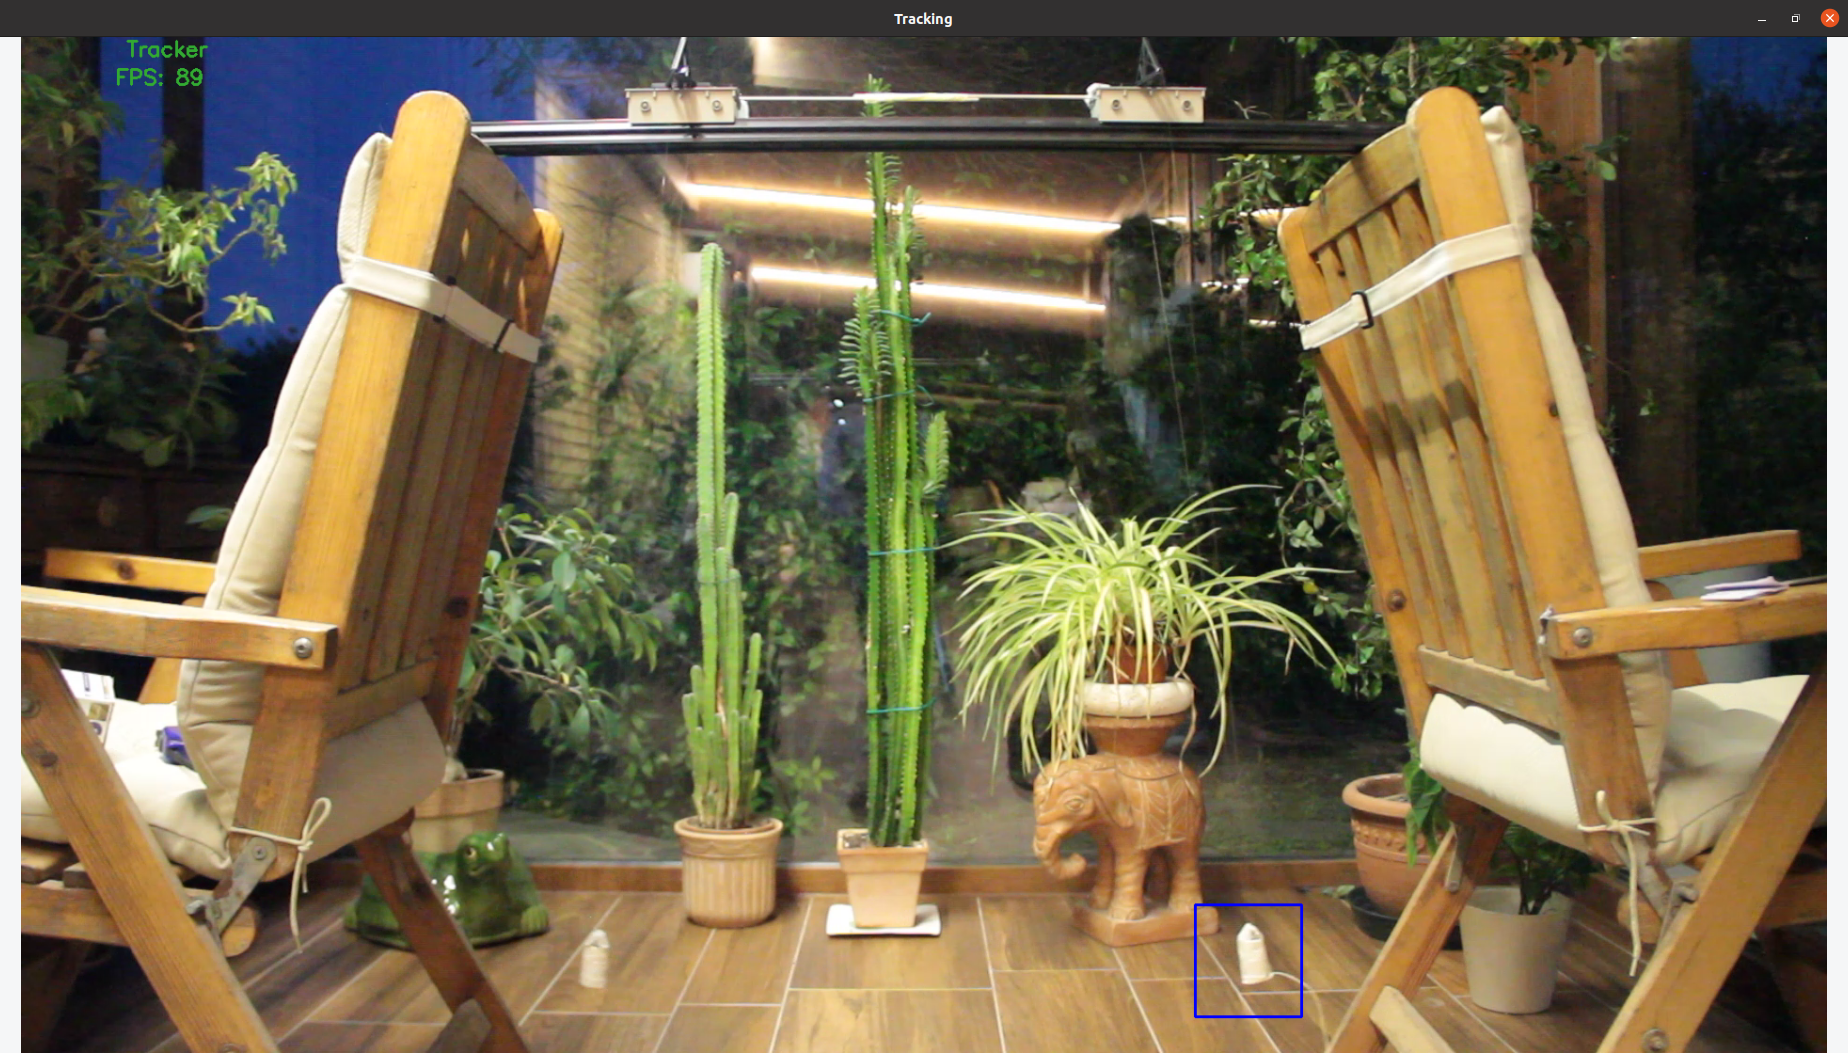
\includegraphics[width=0.9\textwidth]{../../media/img/tracking_2.png}
\end{minipage}
\begin{minipage}{0.3\textwidth}
  \centering
  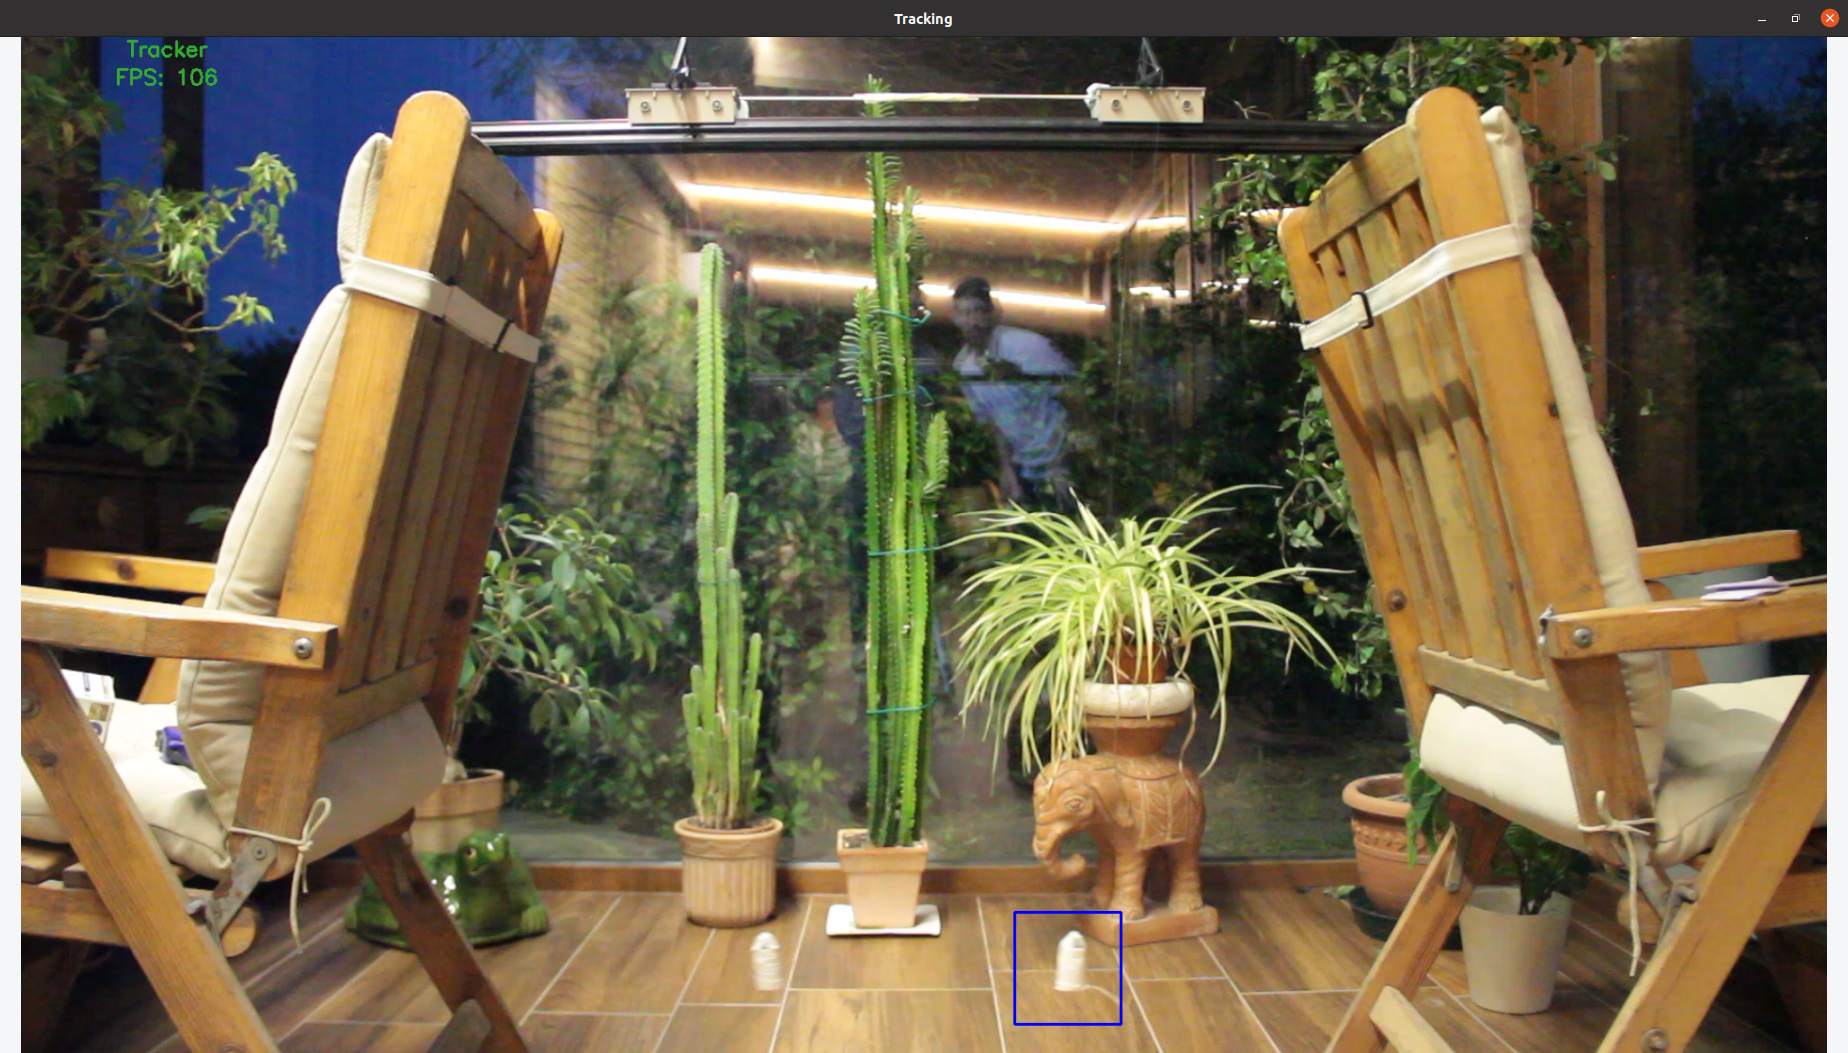
\includegraphics[width=0.9\textwidth]{../../media/img/tracking_3.png}
\end{minipage}
\caption{\textit{Tre istanti del processo di tracking dell'oggetto.
Nell'immagine a destra si osserva il momento di selezione del pendolo, tracciando un rettangolo blu attorno 
allo stesso. Nelle altre due immagini sono mostrati due screenshot effettuati alla 
finestra di tracking, mentre l'algoritmo traccia l'oggetto desiderato, spostando il rettangolo blu.
Nell'immagine a destra si nota anche un istante del processo di rilascio descritto in \cref{sezione_realizz}}}
\label{photo_tracking}
\end{figure}
L'utente può e deve fermare l'acquisizione nel caso noti che il rettangolo
scompaia, accompagnato dal messaggio \textit{Tracking failure detected}, relativo al
caso in cui l'algoritmo non riesca a identificare la posizione dell'oggetto
in un determinato frame.

In seguito all'acquisizione di vari set dati, nel nostro caso 4 per ogni oggetto,
per cercare di limitare eventuali errori di posizione, è stata fatta 
una media tramite il programma in \cref{listatoavg}, stavolta scritto
in python per elasticità nella gestione dei dati in lettura e scrittura.
Sono così stati prodotti quattro files finali, uno per ogni elemento mobile.

Infine, nel listato in \cref{listatoplotter}, sono stati letti i quattro
files citati sopra, e sono stati poi ricavati con considerazioni
trigonometriche gli angoli indicati in \cref{pendolicorpolibero} come
$\theta_1$ e $\theta_2$. Sono quindi stati scelti degli intervalli 
temporali appropriati per effettuare i fit di funzioni del tipo presentato in 
\cref{equazionefinaleh,equazionefinaleq}, in particolare scartando 
i punti iniziali in cui l'apparecchio è fermo, oppure gli ultimi 
qualora il fenomeno da osservare non fosse più presente.

\section{Risultati e discussione}
Il grafico degli angoli $\theta_1$ e $\theta_2$ di \cref{pendolicorpolibero} 
al trascorrere del tempo, mediato sul 
numero di acquisizioni effettuate, è mostrato in
\cref{angles_full}, mentre è presente uno zoom sugli istanti iniziali in \cref{anlges_accurate},
e uno zoom sui massimi in \cref{angles_decrease}, in cui i punti sono stati collegati 
da linee continue.

\begin{figure}[h!]
  \centering
  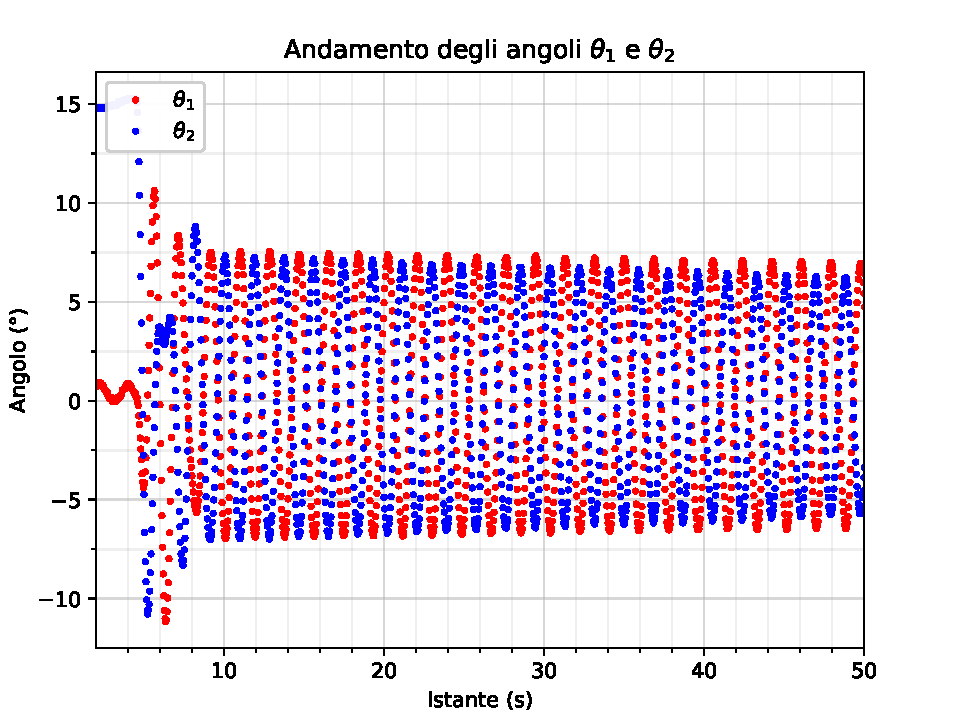
\includegraphics[width=0.8\textwidth]{../../media/plot/angles_full.pdf}
  \caption{\textit{Grafico completo dei due angoli $\theta_1$ e $\theta_2$ al trascorrere del tempo.} }
  \label{angles_full}
\end{figure}

\begin{figure}[h!]
  \centering
  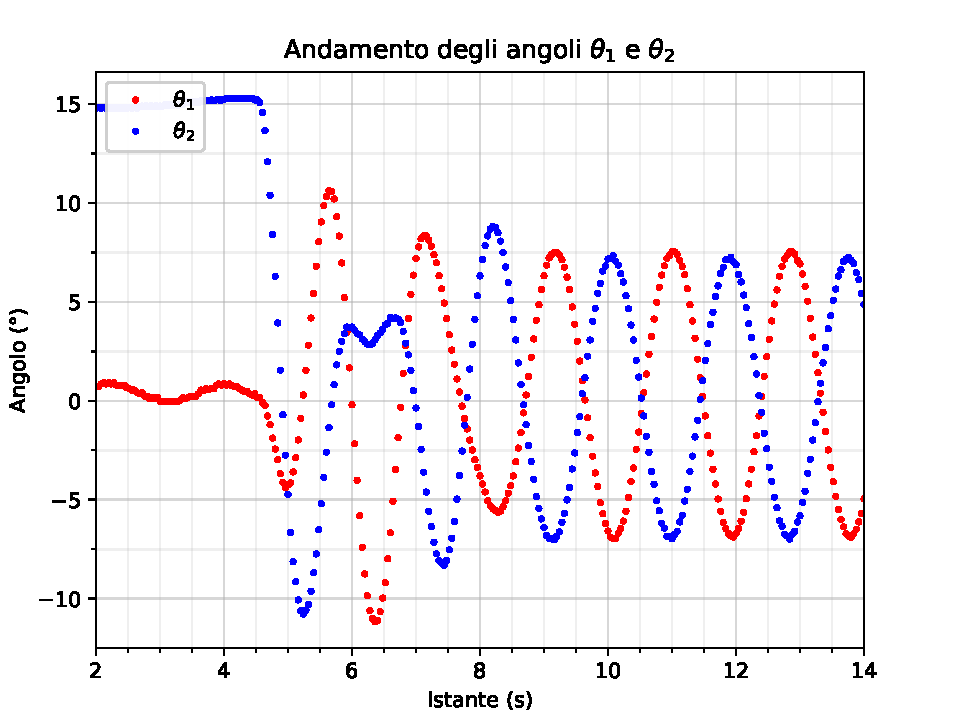
\includegraphics[width=0.8\textwidth]{../../media/plot/angles_accurate.pdf}
  \caption{\textit{Grafico dei due angoli $\theta_1$ e $\theta_2$ al trascorrere del tempo. Zoom sugli istanti iniziali.} }
  \label{anlges_accurate}
\end{figure}

\begin{figure}[h!]
  \centering
  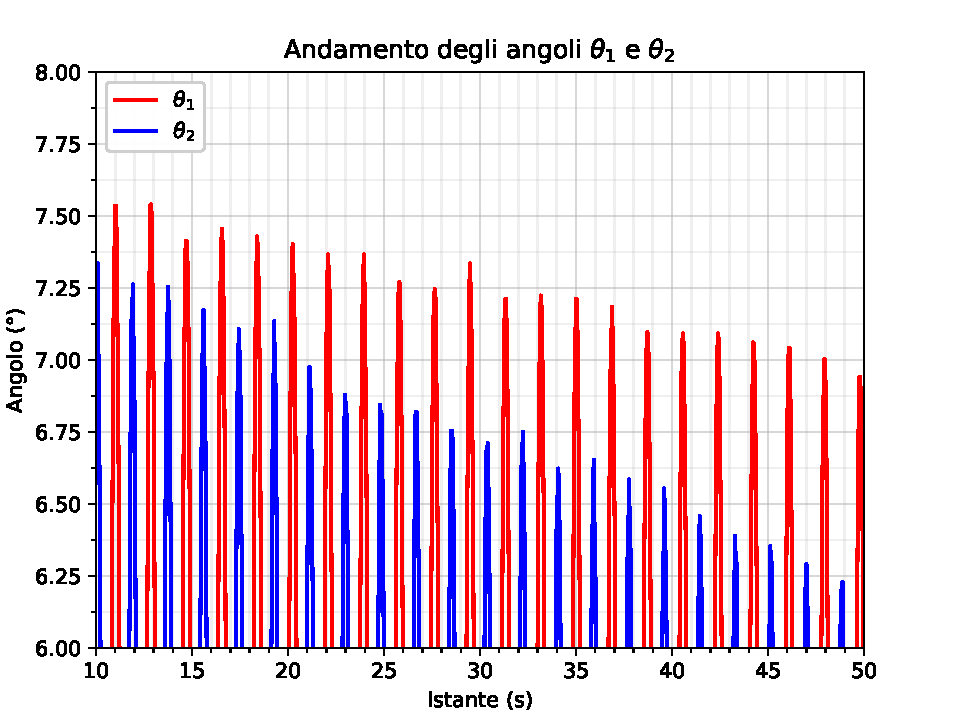
\includegraphics[width=0.8\textwidth]{../../media/plot/angles_decrease.pdf}
  \caption{\textit{Grafico dei due angoli $\theta_1$ e $\theta_2$
  al trascorrere del tempo. Dettaglio delle creste. Si nota come la diminuzione delle ampiezze
  sia di intensità differente.} }
  \label{angles_decrease}
\end{figure}

In \cref{angles_full} si nota come, dopo un breve periodo iniziale di quiete, in cui il
pendolo $\mathbf{P}_1$ si trova in quiete, mentre il pendolo $\mathbf{P}_2$ descrive piccole
oscillazioni dell'ampiezza di circa 1°, che si è cercato di ridurre il più possibile manualmente,
il sistema viene lasciato libero di evolvere: il dettaglio è presente in \cref{anlges_accurate}.
Dopo un momento di transizione, in cui i pendoli e i carrellini descrivono il loro complicato moto,
circa dall'istante 4.6 all'istante 8.5, il sistema mantiene il suo moto nella condizione di
oscillazioni in controfase, quindi con i carrellini necessariamente fermi, per la conservazione
della quantità di moto iniziale, nulla. I pendoli quindi sono stati sincronizzati.
È facile osservare come $\mathbf{P}_1$, che parte da fermo, non ha delle oscillazioni
centrate sugli 0°, errore probabilmente dovuto al tracciamento effettuato in prospettiva.
Si tratta di un errore che, seppur minimo, è sistematico e si continua a manifestare in tutto il moto, 
con la traslazione verso l'alto di tutto il grafico di circa 1°.
Nella \cref{angles_decrease}, dove i punti sono stati collegati da una linea continua nell'
intento di essere più chiari, si nota come sia presente un'evidente differenza nelle oscillazioni 
dei due pendoli: l'ampiezza del pendolo $\mathbf{P}_2$ risulta decrescere più rapidamente rispetto
all'altra: un probabile effetto di un maggiore attrito influente sul pendolo stesso, ad esempio
a livello del perno. Non si tratta infatti di un offset prospettico in quanto dalla \cref{angles_full}
è evidente come la diminuzione dell'ampiezza sia presente simmetricamente, anche a livello dei
minimi di oscillazione.

Possono quindi essere costruite e analizzate le variabili $h$ e $q$, definite nel sistema \labelcref{definizionehq}
e mostrate al variare del tempo nelle \cref{fit_h,fit_q}.
In queste due figure sono anche presenti i due fit delle equazioni teoriche che dovrebbero regolare,
secondo le ipotesi indicate in \cref{sezioneattrito}, il moto delle due variabili, ossia le \cref{equazionefinaleh,equazionefinaleq}.
In basso nelle figure sono mostrati anche i residui, ossia la differenza
, calcolata punto per punto, tra i valori del fit e quelli dei punti acquisiti.
\begin{figure}[h!]
  \centering
  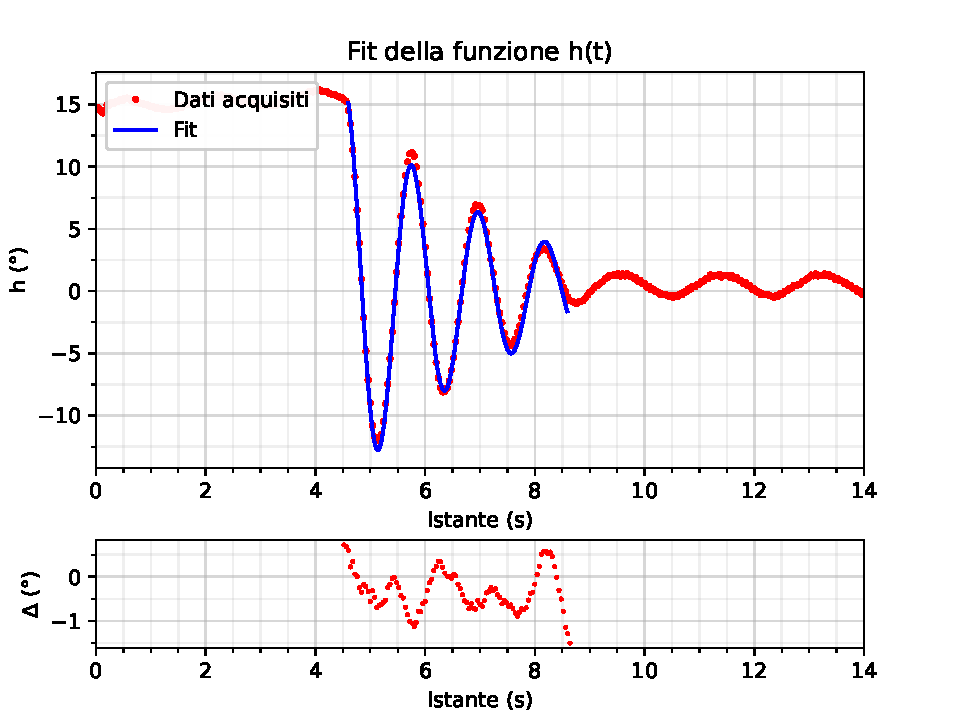
\includegraphics[width=0.8\textwidth]{../../media/plot/fit_h.pdf}
  \caption{\textit{Modello del sistema costruito con indicate
   le grandezze rilevanti. Le lettere maiuscole in grassetto indicano dei punti, quelle in corsivo delle 
   costanti; le minuscole invece indicano le variabili. In basso il grafico dei residui.} }
  \label{fit_h}
\end{figure}

\begin{figure}[h!]
  \centering
  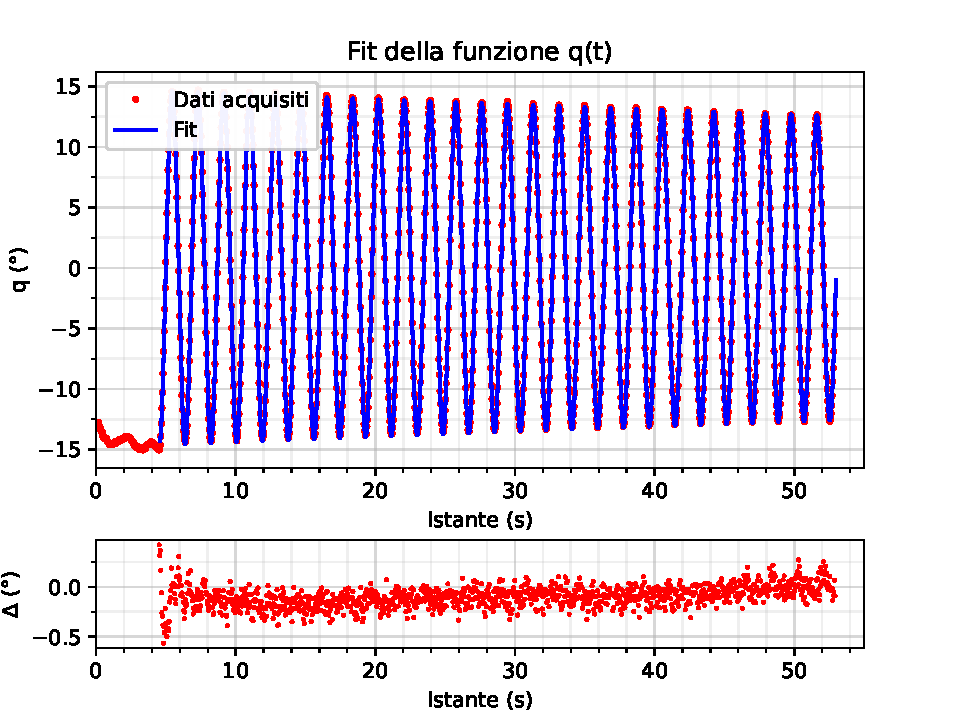
\includegraphics[width=0.8\textwidth]{../../media/plot/fit_q.pdf}
  \caption{\textit{Modello del sistema costruito con indicate
   le grandezze rilevanti. Le lettere maiuscole in grassetto indicano dei punti, quelle in corsivo delle 
   costanti; le minuscole invece indicano le variabili. In basso il grafico dei residui.} }
  \label{fit_q}
\end{figure}

È evidente come non siano presenti pattern che possano dare l'idea di un qualche effetto
sistematico che si potrebbe star trascurando; invece si può ragionevolmente ipotizzare la sola 
presenza di errori casuali, anche dovuti all'imprecisione del metodo di acquisizione, come si nota
dalla distribuzione più o meno casuale dei punti.

Alcuni dubbi sorgono osservando la \cref{fit_h}
, in particolare gli istanti successivi agli \SI{8}{\s}: sembra permanga un'oscillazione
residua, che si traduce in una non esatta sincronia nel movimento dei pendoli; 
praticamente quando un pendolo si trova in una posizione l'altro non si trova nella 
posizione simmetrica, ma leggermente spostato da questa.
L'origine di questo fenomeno non sembra essere dovuto al differente
attrito presente sui due perni, mostrato in \cref{angles_decrease}, in quanto
l'oscillazione residua si mantiene anche al diminuire dell'ampiezza delle
oscillazioni del pendolo più smorzato; il fenomeno potrebbe invece essere 
provocato dalla minima differenza di lunghezza 
dei pendoli, o semplicemente dalla predominanza di fenomeni di attrito statico 
su quelli dinamici.
Infatti, quando i carrellini si fermano, circa agli \SI{8.5}{\s}, interviene non
più l'attrito dinamico ma quello statico, che è caratterizzato da una maggiore intensità
è quindi immune a minime deviazioni che si potrebbero manifestare nella asincronia del moto.

Per quanto riguarda gli errori sulle acquisizioni di posizione, questi non sono stati
stimati a causa della mancanza di informazioni sulla confidenza dell'algoritmo di tracking.

I parametri delle funzioni $h(t)$ \labelcref{equazionefinaleh} e $q(t)$ \labelcref{equazionefinaleq}, stimati dal fit, sono elencati rispettivamente 
nelle \cref{parametrih,parametriq}.
In tabella è indicata anche la somma degli scarti quadratici tra il fit e i punti, il
$\chi^2_h$, indicatore numerico della bontà del fit.
\begin{table}[h!]
  \centering
\begin{minipage}{0.45\linewidth}
  \centering
  \begin{tabular}{cc}
      \toprule
      \multicolumn{2}{c}{Parametri $h(t)$} \\ 
      \midrule
      $A_h$     & \ang{92 \pm 5} \\
      $\gamma_h$& \SI{0.77 \pm 0.02}{\hertz} \\
      $\omega_h$& \SI{5.17 \pm 0.01}{\hertz}\\
      $\beta_h$   &  \SI{1.63 \pm 0.06}{}  \\
      $\chi^2_h$   &  \SI{29.6}{}  \\
      \midrule
    \end{tabular}
  \caption{\textit{Parametri ottenuti dal fit della funzione $h(t)$ \labelcref{equazionefinaleh}.}}
  \label{parametrih}
\end{minipage}
\begin{minipage}{0.45\linewidth}
  \centering
    \begin{tabular}{cc}
        \toprule
        \multicolumn{2}{c}{Parametri $q(t)$} \\ 
        \midrule
        $A_q$     & \ang{14.85 \pm 0.01} \\
        $\gamma_q$& \SI{0.00631 \pm 0.00006}{\hertz} \\
        $\omega_q$& \SI{3.40231 \pm 0.00003}{\hertz}\\
        $\beta_q$   &  \SI{0.275 \pm 0.001}{}  \\
        $\chi^2_q$   &  \SI{26.1}{}  \\
        \midrule
      \end{tabular}
    \caption{\textit{Parametri ottenuti dal fit della funzione $q(t)$ \labelcref{equazionefinaleq}.}}
    \label{parametriq}
\end{minipage}
\end{table}
In realtà il fit è stato effettuato anche con un ulteriore grado di libertà, aggiungendo
un parametro responsabile della traslazione dei grafici delle funzioni rispetto 
all'asse $y$; questo non è stato però riportato in quanto per il miglior fit
tale parametro restava nullo.

Calcolando poi i valori delle frequenze $\omega$, definite in \cref{sezionesenzaattrito},
si ottiene:
$$
\omega_h = \SI{5.62 \pm 0.04}{\hertz}
$$
$$
\omega_q = \SI{3.40 \pm 0.02}{\hertz}
$$
dati che risultano essere in accordo quasi soddisfacente con i risultati del fit delle \cref{parametrih,parametriq}.
È presente una maggiore discordanza per quanto riguarda $\omega_h$, dell'8\%, dovuta 
alle varie sorgenti di errore citate in precedenza ma anche al minor numero di punti disponibili
per il fit.

Notiamo infine che la stima dei coefficienti di attrito data dal fit è in accordo 
con l'idea intuitiva legata alla caratteristica del modo di oscillazione in cui il carrello 
è fermo, ossia alla minor dissipazione di energia rispetto a quello in cui il carrello oscilla in opposizione di 
fase rispetto ai pendoli; ciò è dovuto soprattutto al maggiore attrito generato
durante lo scorrimento sulla rotaia che si somma al normale attrito generato sul perno 
dalle oscillazioni dei pendoli. Questa sorgente di attrito è circa di 2 ordini di grandezza superiore 
rispetto all'altra.
\section{Conclusioni}
In conclusione, è stata osservata con successo la sincronizzazione di due pendoli, ossia la 
 diminuzione dell'ampiezza a zero di un modo normale di oscillazione del sistema, fatto dovuto a differenti
tassi di dissipazione di energia nei due modi appena citati. I due coefficienti $\gamma_h$ 
e $\gamma_q$ sono stati stimati essere pari rispettivamente a \SI{0.77 \pm 0.02}{\hertz} e 
\SI{0.00631 \pm 0.00006}{\hertz}.

\section{Appendice}
Nei seguenti listati sono presenti i file con i quali sono stati estratti 
e visualizzati i dati dell'esperimento.
\subsection{Listato del programma di tracking (C++)}
\lstinputlisting[language=C++]{../c++/tracking.cpp}
\label{listatocpp}
\subsection{Listato del programma di elaborazione dei dati (python)}
\lstinputlisting[language=Python]{../python/avg.py}
\label{listatoavg}
\subsection{Listato del programma di fit e visualizzazione dati (python)}
\lstinputlisting[language=Python]{../python/plotter.py}
\label{listatoplotter}

\end{document}
